%%%%%%%%%%%%%%%%%%%%%%%%%%%%%%%%%%%%%
%                                   %
% Compile with XeLaTeX and biber    %
%                                   %
% Questions or comments:            %
%                                   %
% joshua dot mcneill at uga dot edu %
%                                   %
%%%%%%%%%%%%%%%%%%%%%%%%%%%%%%%%%%%%%

\documentclass{beamer}
  % Read in standard preamble (cosmetic stuff)
  %%%%%%%%%%%%%%%%%%%%%%%%%%%%%%%%%%%%%%%%%%%%%%%%%%%%%%%%%%%%%%%%
% This is a standard preamble used in for all slide documents. %
% It basically contains cosmetic settings.                     %
%                                                              %
% Joshua McNeill                                               %
% joshua dot mcneill at uga dot edu                            %
%%%%%%%%%%%%%%%%%%%%%%%%%%%%%%%%%%%%%%%%%%%%%%%%%%%%%%%%%%%%%%%%

% Beamer settings
% \usetheme{Berkeley}
\usetheme{CambridgeUS}
% \usecolortheme{dove}
% \usecolortheme{rose}
\usecolortheme{seagull}
\usefonttheme{professionalfonts}
\usefonttheme{serif}
\setbeamertemplate{bibliography item}{}

% Packages and settings
\usepackage{fontspec}
  \setmainfont{Charis SIL}
\usepackage{hyperref}
  \hypersetup{colorlinks=true,
              allcolors=blue}
\usepackage{graphicx}
  \graphicspath{{../../figures/}}
\usepackage[normalem]{ulem}
\usepackage{enumerate}

% Document information
\author{M. McNeill}
\title[FREN2001]{Français 2001}
\institute{\url{joshua.mcneill@uga.edu}}
\date{}

%% Custom commands
% Lexical items
\newcommand{\lexi}[1]{\textit{#1}}
% Gloss
\newcommand{\gloss}[1]{`#1'}
\newcommand{\tinygloss}[1]{{\tiny`#1'}}
% Orthographic representations
\newcommand{\orth}[1]{$\langle$#1$\rangle$}
% Utterances (pragmatics)
\newcommand{\uttr}[1]{`#1'}
% Sentences (pragmatics)
\newcommand{\sent}[1]{\textit{#1}}
% Base dir for definitions
\newcommand{\defs}{../definitions}


  % Packages and settings

  % Document information
  \subtitle[Activités]{Les activités, les verbes \lexi{-er} et la négation}

\begin{document}
  % Read in the standard intro slides (title page and table of contents)
  \begin{frame}
    \titlepage
    \tiny{Office: % Basically a variable for office hours location
Gilbert 121\\
          Office hours: % Basically a variable for office hours
 lundi, mercredi, vendredi 10:10--11:10
}
  \end{frame}

  \begin{frame}{Annonces}
    \begin{itemize}
      \item L'atelier d'écoute, le 11 septembre
      \item[] \tinygloss{Listening workshop, September 11th}
      % \item Rendez le devoir 1, le 11 septembre
      % \item[] \tinygloss{Turn in homework, September 11th}
    \end{itemize}
  \end{frame}

  \begin{frame}{}
    \begin{center}
      \Large Quiz
    \end{center}
  \end{frame}

  \begin{frame}{Révision des verbes \lexi{-er}}
    Par exemple:
    \begin{center}
      \begin{tabular}{l | l l | l l}
  \multicolumn{5}{c}{regarder \gloss{to look at, to watch}} \\
      & \multicolumn{2}{l |}{singulier} & \multicolumn{2}{l}{pluriel} \\
  \hline
  1re & je         & regarde            & nous        & regardons \\
  2e  & tu         & regardes           & vous        & regardez \\
  \hline
  3e  & il (masc)  &                    & ils (masc)  & \\
      & elle (fem) & regarde            & elles (fem) & regardent \\
      & on         &                    &             & \\
\end{tabular}

    \end{center}
  \end{frame}

  \begin{frame}{Affirmation et négation}
    Quelle est la bonne conjugation? \\
    \tinygloss{What is the correct conjugation?}
    \begin{columns}
      \column{0.5\textwidth}
        \begin{enumerate}
          \item J'\underline{\uncover<2->{invite}} (inviter) mes parents.
          \item On ne \underline{\uncover<4->{regarde}} (regarder) pas la télé.
          \item Elle n'\underline{\uncover<6->{aime}} (aimer) pas le tennis.
          \item Ils \underline{\uncover<8->{habitent}} (habiter) à la maison.
          \item Nous \underline{\uncover<10->{retrouvons}} (retrouver) nos amis.
          \item Vous ne \underline{\uncover<12->{travaillez}} (travailler) pas au restaurant.
        \end{enumerate}
      \column{0.5\textwidth}
        \begin{minipage}[c][0.6\textheight]{\linewidth}
          \begin{center}
            \only<1-2>{
              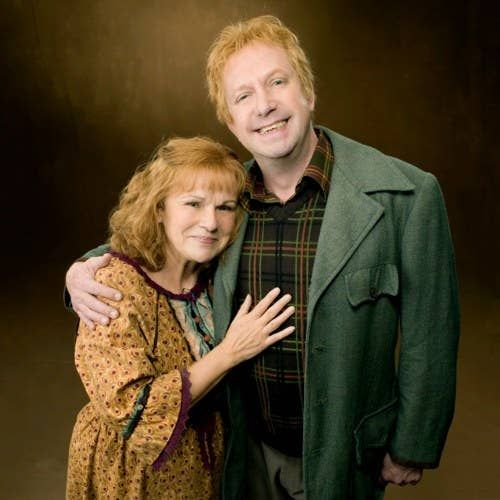
\includegraphics[scale=0.3]{weasley.jpg}
            }
            \only<3-4>{
              
\includegraphics[scale=0.09]{television.jpg}
            }
            \only<5-6>{
              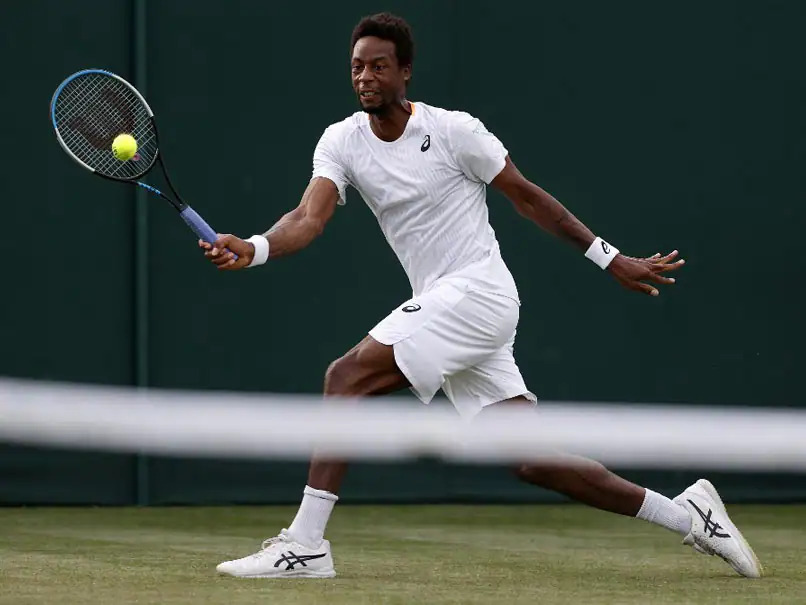
\includegraphics[scale=0.2]{monfils.jpg} \\
              Gaël Monfils
            }
            \only<7-8>{
              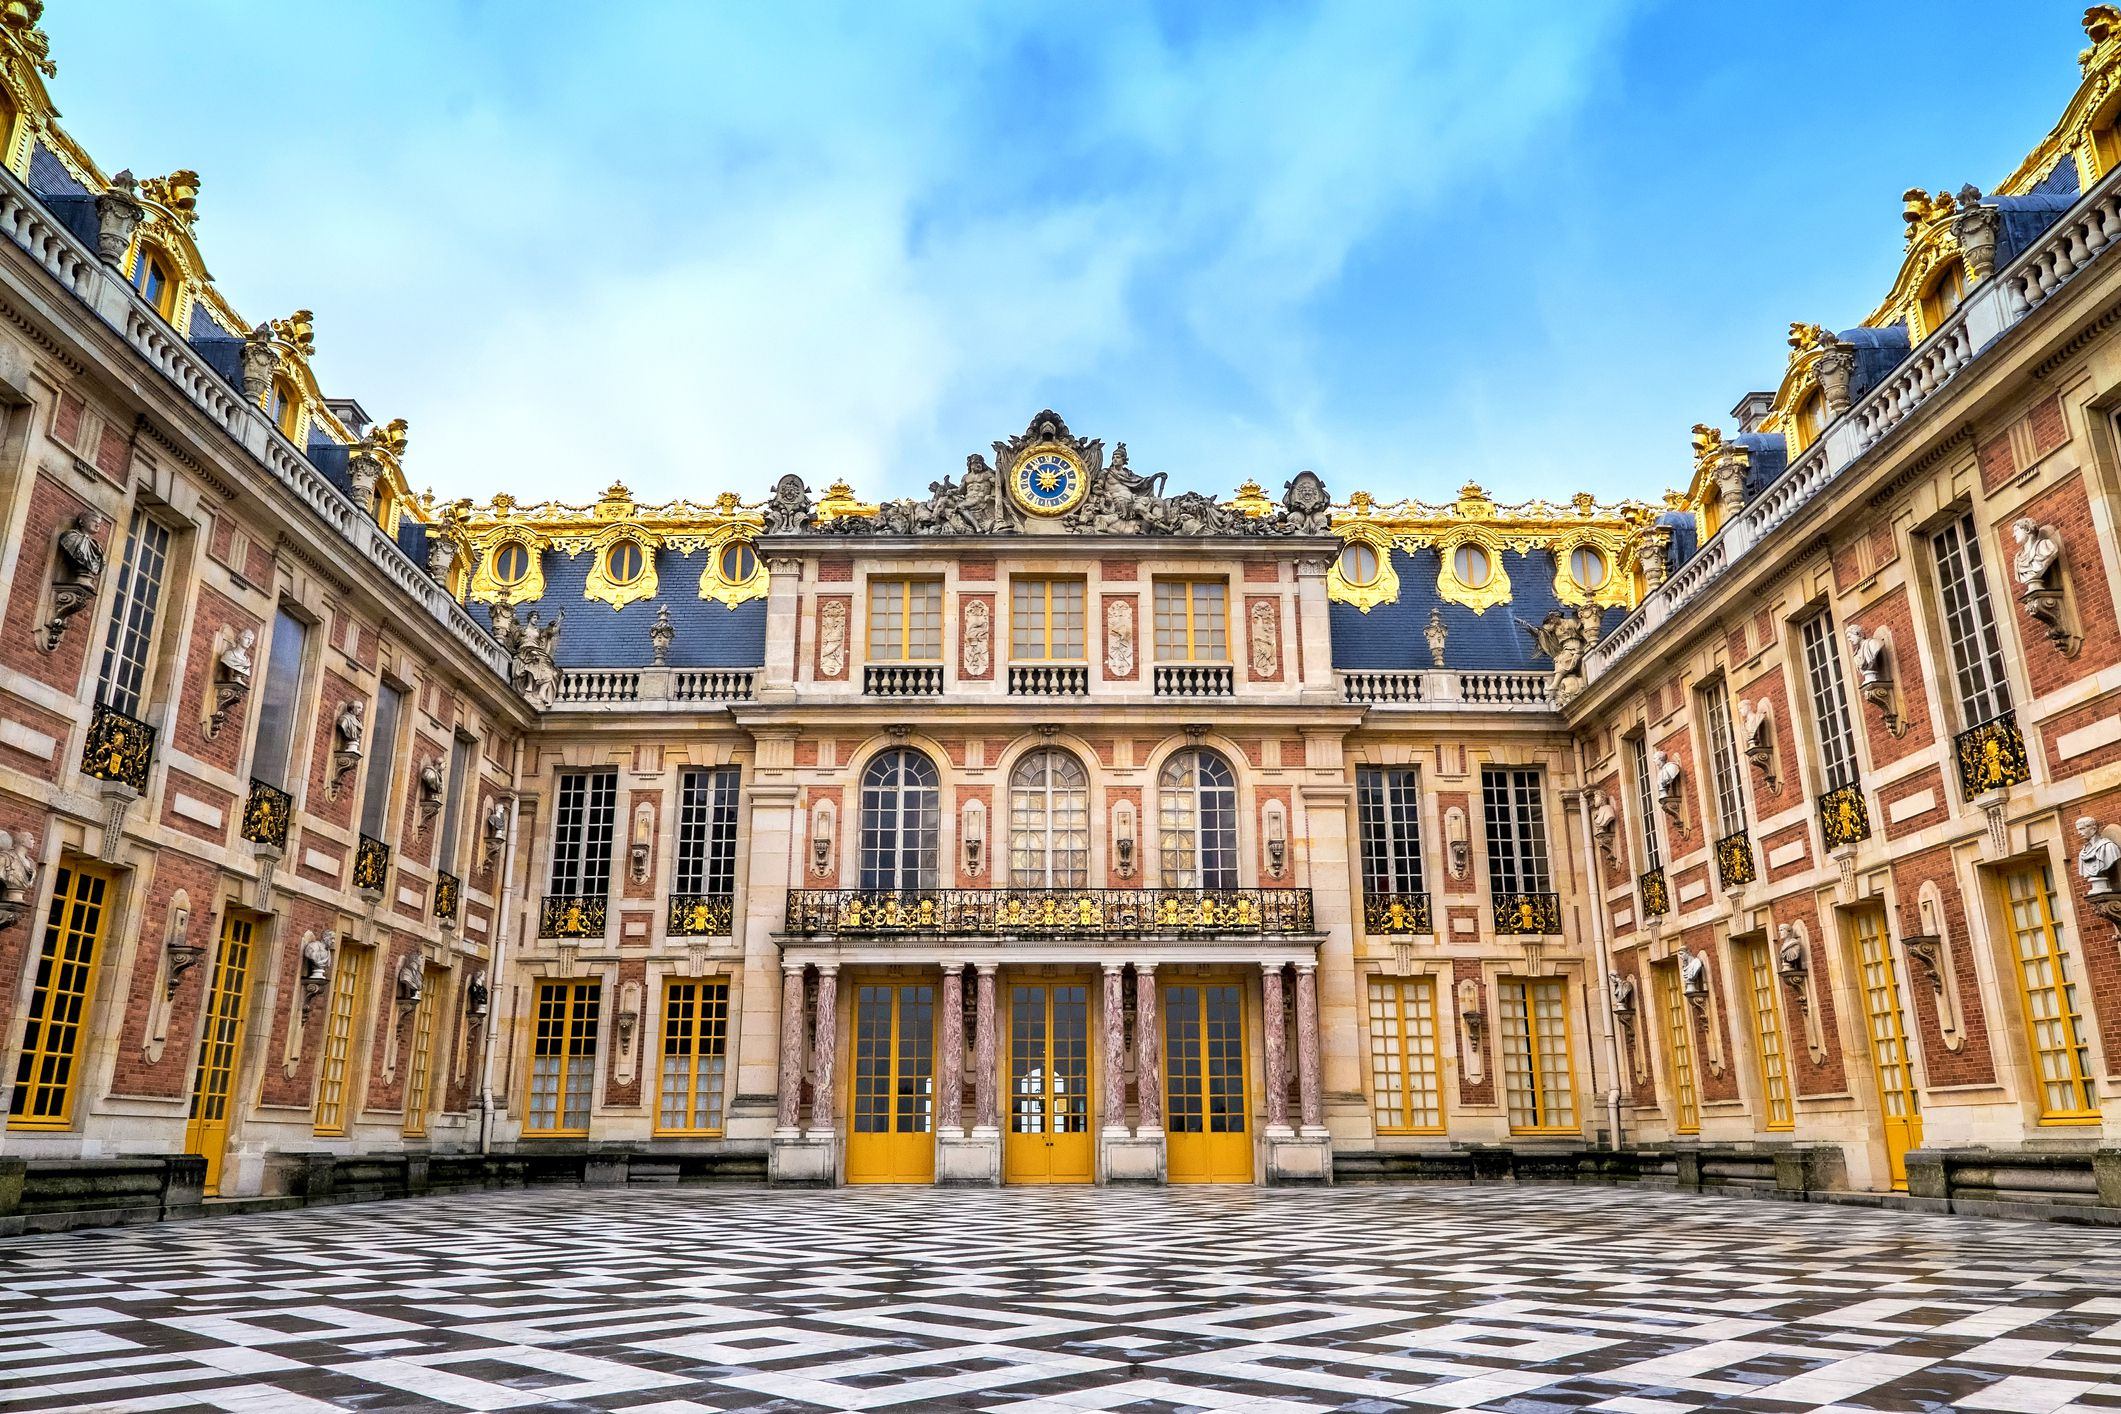
\includegraphics[scale=0.08]{versailles.jpg} \\
              Le château de Versailles
            }
            \only<9-10>{
              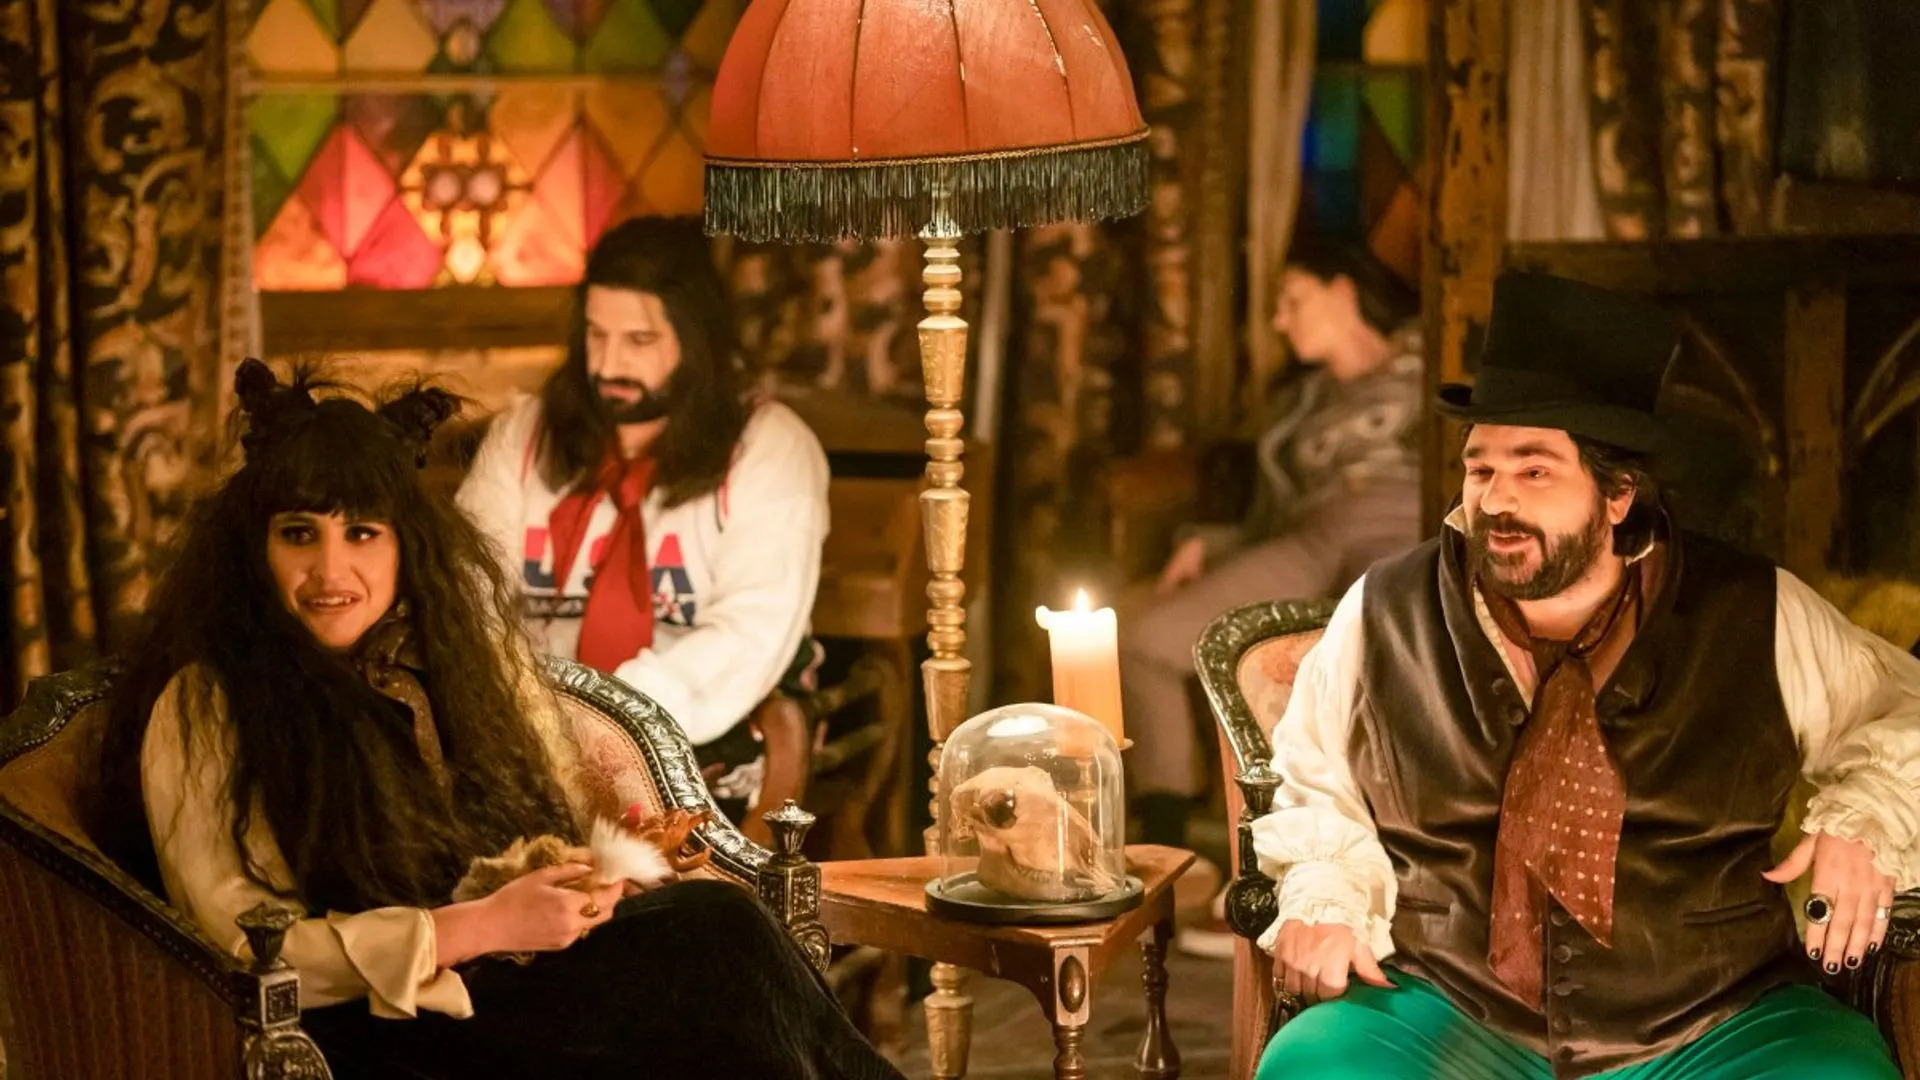
\includegraphics[scale=0.09]{amis.jpg}
            }
            \only<11-12>{
              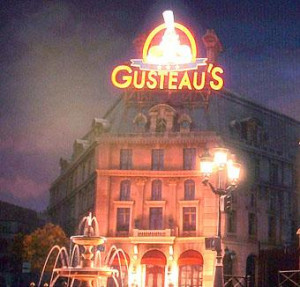
\includegraphics[scale=0.7]{gusteau.jpg}
            }
            \only<13->{
              \begin{itemize}
                \item Des mots associés à \lexi{regarder}
                \item[$\to$] la télé, un film, le tableau
                \item[] \tinygloss{Some words associated with \lexi{regarder}}
                \item[] \tinygloss{$\to$ la télé, un film, le tableau}
              \end{itemize}
            }
          \end{center}
        \end{minipage}
    \end{columns}
  \end{frame}

  \begin{frame}{Les associations des verbes \lexi{-er}}
    \centering
    écouter

    \uncover<2->{
      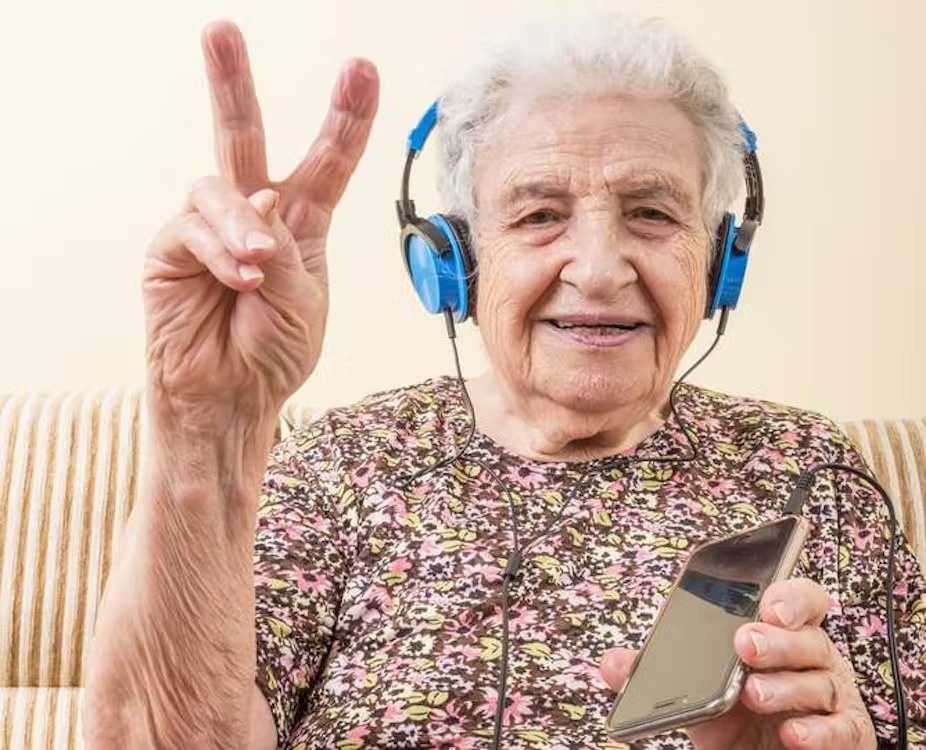
\includegraphics[scale=0.2]{ecouter.jpg}
    }
  \end{frame}

  \begin{frame}{Les associations des verbes \lexi{-er}}
    \centering
    jouer

    \uncover<2->{
      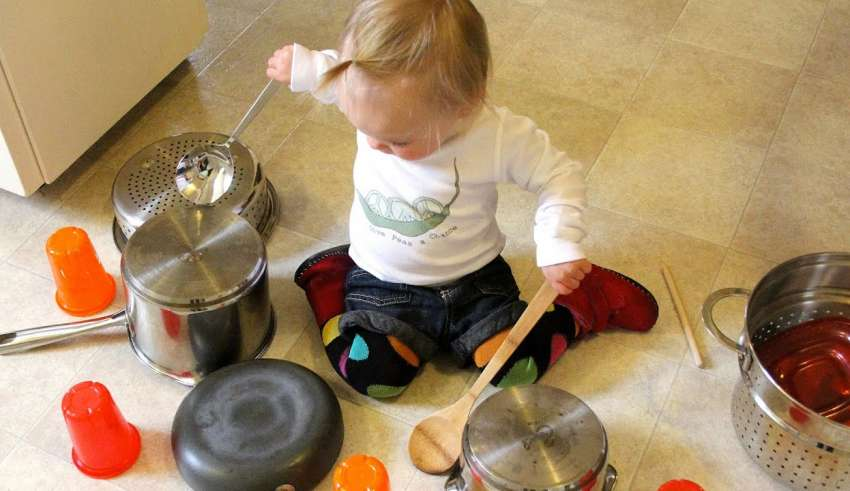
\includegraphics[scale=0.4]{jouer.jpg}
    }
  \end{frame}

  \begin{frame}{Les associations des verbes \lexi{-er}}
    \centering
    préparer

    \uncover<2->{
      \includegraphics[scale=1]{préparer.jpg}
    }
  \end{frame}

  \begin{frame}{Les associations des verbes \lexi{-er}}
    \centering
    parler

    \uncover<2->{
      
\includegraphics[scale=0.25]{parler.jpg}
    }
  \end{frame}

  % \begin{frame}{Les associations des verbes \lexi{-er}}
  %   \centering
  %   travailler

  %   \uncover<2->{
  %     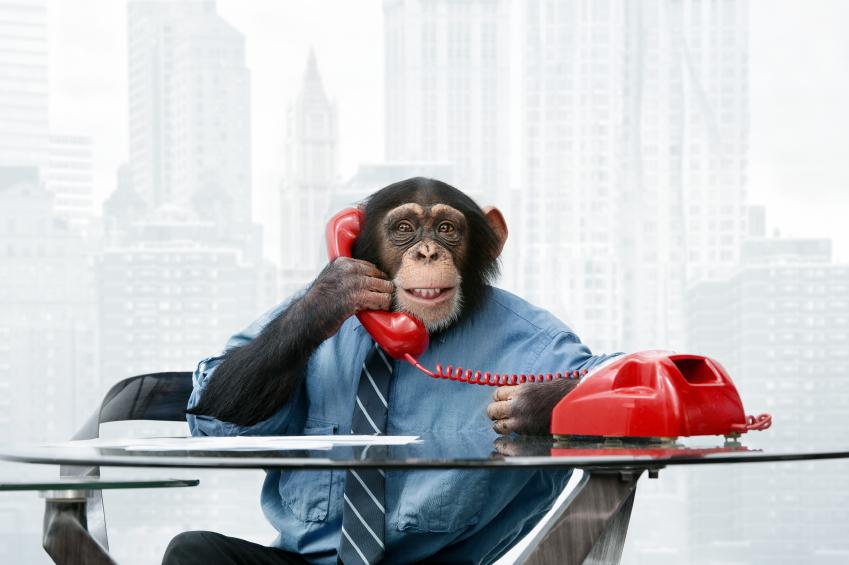
\includegraphics[scale=0.75]{travailler.jpg}
  %   }
  % \end{frame}

  % \begin{frame}{Les associations des verbes \lexi{-er}}
  %   \begin{columns}
  %     \column{0.5\textwidth}
  %       \begin{center}
  %         inviter
  %       \end{center}
  %     \column{0.5\textwidth}
  %       \begin{center}
  %         \uncover<2->{
  %           
\includegraphics[scale=0.37]{inviter.jpg}
  %         }
  %       \end{center}
  %   \end{columns}
  % \end{frame}

  \begin{frame}{Habitudes \gloss{Habits}}
    Avec un/e partenaire, parle de ce que vous faites quelquefois.
    Donne des exemples en combinant les verbes suivants avec du vocabulaire, et dis à ton/ta partenaire si tu fais les mêmes choses que lui/elle. \\
    \tinygloss{With a partner, talk about what you sometimes do.
    Give some examples by combining the following verbs with the vocabulary, and tell your partner if you do the same things as them.}
    % \vspace{0.2cm}
    \begin{columns}[t]
      \column{0.3\textwidth}
        \begin{enumerate}
          \item[] \textbf{Verbes:}
          \item travailler
          \item écouter
          \item jouer
          \item réviser
          \item regarder
          \item préparer
          \item inviter
        \end{enumerate}
      \column{0.7\textwidth}
        \begin{description}
          \item[] \textbf{Modèle:}
          \item[E1:] Je téléphone à ma mère.
          \item[] \tinygloss{I call my mother.}
          \item[E2:] Moi, je ne téléphone pas à ma mère.
          \item[] \tinygloss{Me, I don't call my mother.}
          \item[OU] Je téléphone à ma mère, aussi \gloss{also}. Nous téléphonons à nos mères.
          \item[] \tinygloss{I call my mother, also. We call our mothers.}
        \end{description}
    \end{columns}
  \end{frame}

  \begin{frame}{Des endroits \gloss{Places}}
    Avec un/e partenaire, dis ce que tu fais à chacun des endroits suivants. \\
    \tinygloss{With a partner, say what you do at each of the following places.}
    \begin{enumerate}
      \item au bureau
      \item à la fac
      \item à la maison
      \item au restaurant
    \end{enumerate}
  \end{frame}

  \begin{frame}{}
    \begin{center}
      \Large Questions?
    \end{center}
  \end{frame}
\end{document}
